\documentclass[11pt,a4paper]{article}

\typeout{------------------------------------------------------------------}
\typeout{} 
\typeout{        Fichier de base modifie par : Matth: 20 nov 2012} 
\typeout{                   sous licence GNU-GPL} 
\typeout{}
\typeout{------------------------------------------------------------------}

% Classe générale du document
   %documentclass[12pt,a4paper]{article} % .10pt, 11pt, 12pt : taille de la police principale (10 par défaut)
                 % .a4paper, letterpaper,... : délimite la taille du papier. (letterpaper par défaut)
	         % .fleqn : aligne les formules mathématiques à gauche au lieu de les centrer.
		 % .leqno : place la numérotation des formules à gauche plutôt qu'à droite.
		 % .twocolumn : demande à LATEX de formater le texte sur deux colonnes.
		 % .twoside, oneside indique si la sortie se fera en recto-verso ou en recto simple.
		 % .landscape, mais il faut mettre en commentaire (ou modifier) toutes les dimmensions

% Importation de packages divers
%   \NeedsTeXFormat{LaTeX2e} 
   \usepackage[T1]{fontenc}
   \usepackage[utf8x]{inputenc}		% utilisation des caractères 8 bits en Unix (codage ISO 8859-1)
  %\usepackage[latin1]{inputenc}	% utilisation des caractères pour Linux2
   \usepackage[usenames]{color}
   \usepackage{fancyhdr}
   \usepackage{lastpage}                % pour l'affichage du n° de la dernière page.
   \usepackage{lmodern}
   \usepackage{multirow}                % pour l'utilisation de figures ``noyées'' dans le texte
   \usepackage{xspace}			% package pour babel
   \usepackage[english]{babel}         % Utilisation du français (nom des sections, césure, ponctuation,...)
   \usepackage[english]{varioref}        % vpageref
   \usepackage{amsmath,amsthm,amssymb}  % Utilisation de certains packages de AMS (cf. belles équations)
   \usepackage{endnotes}                % Pour l'utilisation des notes en fin de documents
   \usepackage{verbatim}                % Pour l'insertion de fichier en mode verbatim
   \usepackage{portland}		% pour l'utilisation de \portrait et de \landscape sur une page
   \usepackage[pdftex]{graphicx}        % [pdftex] si utilisation d'images jgp,...
                                        % [dvips]  si utilisation d'images bmp,...
   \usepackage{pdfpages}		% Inclure des pages de pdf
   \usepackage{pdflscape}		% rotate => begin{landscape} ... \end{landscape}
   \usepackage{setspace}		% Pour définir un interligne
   \usepackage{tkz-orm}
   \usepackage[bottom]{footmisc}        % Footnote at the bottom
%   \usepackage[cyr]{aeguill}		% Pour les guillemets à la Française
   \usepackage{eurosym}			% Pour les Euro
   \usepackage{url}
    \urlstyle{sf}
   \usepackage[backgroundcolor=yellow]{todonotes} %% todonotes: \listoftodos & \todo{Some note or other.} & \missingfigure{}
	
   \renewcommand{\contentsname}{Sommaire} % si tableofcontents au début
   \newcommand{\Numero}{\No}
   \newcommand{\numero}{\no}
%   \newcommand{\fup}[1]{\up{#1}}

   \DeclareGraphicsExtensions{.jpg,.pdf,.mps,.png}       % déclaration d'extensions  pour les images
   %\input xy                            % pour le package xy (construction de diagramme)
   %\xyoption{all}

% Dimensions de la page :       	

  %%%%%%%%%%%%%%%%%%%%%%%%%%%%%%%%%%%%%%%%  0
  %   |                                  %
  %---+----------------------------------%  1
  %   | +----------------------------+   %  2
  %   | |          en-tête           |   %
  %   | +----------------------------+   %  3
  %   | +----------------------------+   %  4
  %   | |                            |   %       Remarques : 
  %   | |                            |   %        . distance de '0' à '1' : un pouce + \voffset
  %   | |                            |   %        . distance de 'a' à 'b' : un pouce + \hoffset
  %   | |           texte            |   %
  %   | |                            |   %
  %   | |                            |   %
  %   | |                            |   %
  %   | +----------------------------+   %  5
  %   | +----------------------------+   %
  %   | |         bas de page        |   %
  %   | +----------------------------+   %  6
  %%%%%%%%%%%%%%%%%%%%%%%%%%%%%%%%%%%%%%%%
  %a  b c                            d  e

%    % général
%      \voffset       0mm    % pour descendre (si positif) ou remonter (si négatif) le tout
%      \hoffset       0mm    % pour agrandir (si positif) ou diminuer (si négatif) la marge gauche (distance 'a' 'b')
%      \oddsidemargin 0mm   % 5pt  % distance de 'b' à 'c'
%     \evensidemargin 25mm  % 15pt % distance de 'd' à 'e'
%    % texte
%      \headsep       25pt   % distance de '3' à '4', la distance entre l'en-tête et le texte
%     \textheight    220mm  % distance de '4' à '5', pour déterminer la hauteur du texte
%     \textwidth     160mm  % distance de 'c' à 'd' 
%    % en-tête
%     \topmargin     0pt    % distance de '1' à '2', pour descendre (si positif) ou remonter (si négatif) le tout
%     \headheight    15pt   % distance de '2' à '3', doit être > 14.49999
%    % bas de page
%     \footskip      15mm   % 30pt % distance de '5' à '6', la distance entre le texte et le bas de page
     % space for the footnode
%    \setlength{\skip\footins}{1cm}

\usepackage[top=2.5cm, bottom=2.5cm, left=2.5cm, right=2.5cm]{geometry}

% (Re)définitions diverses

  % redéfinition de l'affichage des titres de section dans l'en-tête ou le bas de page
    % remarques :
    %  .affichage du numéro (2)    : \thesection 
    %  .affichage du nom (Section) : \sectionname
   % \renewcommand{\sectionmark}[1]{\markright{\thesection.\ #1}}   % 2.2. nom de la section 2.2
   % \renewcommand{\thesection}{\arabic{section}}		% II nom de la section 0.2


  % des couleurs...                   (utilisation avec par ex. \textcolor{webdarkblue}{...})
   \definecolor{codeBlue}{rgb}{0,0,1}
   \definecolor{webred}{rgb}{0.5,0,0}
   \definecolor{codeGreen}{rgb}{0,0.5,0}
   \definecolor{codeGrey}{rgb}{0.6,0.6,0.6}
   \definecolor{webdarkblue}{rgb}{0,0,0.4}
   \definecolor{webgreen}{rgb}{0,0.3,0}
   \definecolor{webblue}{rgb}{0,0,0.8}
   \definecolor{orange}{rgb}{0.7,0.1,0.1}

  % utilisation de caption, label,... pour autre chose qu'une figure
        %%%% debut macro %%%%
   \makeatletter
   \def\captionof#1#2{{\def\@captype{#1}#2}}
   \makeatother
        %%%% fin macro %%%%


% remarques : 
%  . pour mettre la date                  : \today
%  . pour mettre le nom de la section     : \rightmark
%  . pour mettre le numéro de page        : \thepage
%  . pour mettre le nombre de pages total : \pageref{LastPage}  (mais l'écrit en rouge vu que c'est une réf.)
%  . insertion d'une image                : \setlength{\unitlength}{1mm}
%                                             \begin{picture}(0,0)
%                                                \put(5,0){\includegraphics[scale=x.x]{xxx.xxx}}
%                                             \end{picture}

% Pour les guillemets à  la Française
\newcommand{\fermerguillemets}{\unskip\kern.15em\symbol{20}}
\newcommand{\ouvrerguillemets}{\symbol{19}\ignorespaces\kern.15em}
% \let »=\fermerguillemets
% \let« =\ouvrerguillemets

% Pour changer l'icone des puces : à placer juste avant une liste
 %   \renewcommand\labelitemi{\textbullet}	% Style boulet :)
\usepackage[pdfusetitle,
	    colorlinks=true,
	    linkcolor=webdarkblue, 
	    filecolor=webblue, 
	    urlcolor=webdarkblue,
	    citecolor=webgreen]{hyperref}     % pour l'utilisation des liens http,...

% Police
   %\renewcommand\familydefault{ptm}        % famille normale: Times ptm
   %\renewcommand\rmdefault{phv}            % famille à utiliser pour du Roman (phv)
   \renewcommand{\familydefault}{\sfdefault}

% L'interligne
%   \onehalfspacing % un et demi (= \setstrech{1.5} ou = \renewcommand{\baselinestretch}{1.5})
%   \renewcommand{\baselinestretch}{1.15}

     
% Mise en page
%   \pagestyle{fancy} %% custom en-tête
%   \usepackage[Matth]{fncychap}

% En-tete
%   \lhead{\texttt{LECGE1321} - Travail de Management Humain}        \chead{}        \rhead{Groupe 74}
%   \renewcommand{\headrulewidth}{0.5pt}     % pour l'épaisseur de la ligne

% Bas de page
%   \renewcommand{\footrulewidth}{0.5pt}       % pour l'épaisseur de la ligne
%   \lfoot{Partie \rightmark}        \cfoot{}        \rfoot{Page \thepage~sur~\pageref*{LastPageModif}}

% TOC jusqu'au subsection
\setcounter{tocdepth}{2} % Dans la table des matieres
\setcounter{secnumdepth}{3} % Avec un numero.

\usepackage{listings}
\lstset{
    language=Ruby,
	breakatwhitespace=true,
	breaklines=true,
	keepspaces=true,
	numbers=left,
	numbersep=5pt,
	showstringspaces=true,
	frame=single,
	basicstyle=\footnotesize,
	title=\lstname,
    literate=
      {á}{{\'a}}1 {é}{{\'e}}1 {í}{{\'i}}1 {ó}{{\'o}}1 {ú}{{\'u}}1
      {Á}{{\'A}}1 {É}{{\'E}}1 {Í}{{\'I}}1 {Ó}{{\'O}}1 {Ú}{{\'U}}1
      {à}{{\`a}}1 {è}{{\'e}}1 {ì}{{\`i}}1 {ò}{{\`o}}1 {ò}{{\`u}}1
      {À}{{\`A}}1 {È}{{\'E}}1 {Ì}{{\`I}}1 {Ò}{{\`O}}1 {Ò}{{\`U}}1
      {ä}{{\"a}}1 {ë}{{\"e}}1 {ï}{{\"i}}1 {ö}{{\"o}}1 {ü}{{\"u}}1
      {Ä}{{\"A}}1 {Ë}{{\"E}}1 {Ï}{{\"I}}1 {Ö}{{\"O}}1 {Ü}{{\"U}}1
      {â}{{\^a}}1 {ê}{{\^e}}1 {î}{{\^i}}1 {ô}{{\^o}}1 {û}{{\^u}}1
      {Â}{{\^A}}1 {Ê}{{\^E}}1 {Î}{{\^I}}1 {Ô}{{\^O}}1 {Û}{{\^U}}1
      {œ}{{\oe}}1 {Œ}{{\OE}}1 {æ}{{\ae}}1 {Æ}{{\AE}}1 {ß}{{\ss}}1
      {ç}{{\c c}}1 {Ç}{{\c C}}1 {ø}{{\o}}1 {å}{{\r a}}1 {Å}{{\r A}}1
      {€}{{\EUR}}1 {£}{{\pounds}}1
}

% Juste pour avoir un titre dans le pdf
\title{Software Development Project - Report 2}
\author{Group 6: Matthieu Baerts, Benoît Baufays, Julien Colmonts, Benjamin Frantzen, Pierre-Yves Légéna, Vincent Van Ouytsel, Ludovic Vannoorenberghe, Alex Vermeylen}

\begin{document}
\begin{titlepage}
\newgeometry{left=2cm,right=2cm,top=2cm,bottom=2cm}

\rm %% style Roman for the title

\begin{center}

% Upper part of the page
%\vspace*{-2cm}

\includegraphics[scale=.5]{ingi.png}\\[2cm]

\textsc{\LARGE Pôle d'ingénierie informatique}\\[1.5cm]

\textsc{\Large \texttt{LSINF2255} - Software Development Project}\\[0.5cm]


% Title
\vspace{3.5cm}
{ \huge \bfseries Requirements analysis report\vspace{0.8cm}}

\vspace{3.5cm}

% Author and supervisor
\begin{minipage}{0.4\textwidth}
\begin{flushleft} \large
\emph{Professor:}\\
	Kim \textsc{Mens}\\
\vspace{1cm}
\emph{Assistant:}\\
	Sergio \textsc{Castro Mejia} % Apple lover
\end{flushleft}
\end{minipage}
\begin{minipage}{0.4\textwidth}
\begin{flushright} \large
\emph{Students: (Group 6 - SINF2MS)} \\
%\begin{tabular}{rr}
	Matthieu \textsc{Baerts}\\
	Benoît \textsc{Baufays}\\
	(\textit{Project Manager}) Julien \textsc{Colmonts}\\
	Benjamin \textsc{Frantzen}\\
	Pierre-Yves \textsc{Légéna}\\
	Vincent \textsc{Van Ouytsel}\\
	Ludovic \textsc{Vannoorenberghe}\\
	Alex \textsc{Vermeylen}
%\end{tabular} \\
\end{flushright}
\end{minipage}

\vfill

% Bottom of the page
{\large Academic Year 2013-2014}
\end{center}

\end{titlepage}
\restoregeometry

\tableofcontents
%\thispagestyle{empty}	% pour enlever le numéro de page
\newpage
%\pagenumbering{arabic} % on triche avec la numéroation des pages :)

\section*{Introduction}
\addcontentsline{toc}{section}{Introduction}
At the begining of this phase, we just received the feedback of the previous one, so we knew the pros and cons of our work.
Looking at these informations, we decided to improve ourselves by taking the remarks in account.
The goals of this part of the job was to go further in the modelisation of the architecture of the program.
To do this, we had to create some diagrams : 
\begin{itemize}
\item A class diagram, showing the differents objects, their attributes, their main methods and the relations linking them.
\item Some sequences diagrams, to illustrate the most important user activities by displaying the interactions between the objects in several defined scenarios.
\item An ORM diagram, to show graphically the fields of the database and its architecture.
\item A box pointer diagram, to explain the way that the modules of the website are working together sequentially on a timeline.
\end{itemize}
Doing all theses diagrams will allow us to have a better overview of the project. So we will have a more precise idea on how the website will run. 
Two others requiered elements in this report were to detail the physical architecture and the framework that we chose and to argue the choice.
We had to do research to justify our choice and have a look on the physical architecture and how the chosen framework imposes it.

\newpage

\section{Architecture Model}
\subsection{Application} %% TODO: another title...

\subsubsection{Class Diagram} %% TODO: another title...
See figure \vref{fig:uml}.\\
The class diagram shows the main classes of the model. Each variable of the class are detailled but only the main specific function that should be implemented are there and to avoid an overloading of the diagram we didn't list all the getters and setters of the variables. The hollow arrow shows the extended classes. For example, the classes Client and CoWorker extend User. The simple arrow shows a link between two classes and the indexes the number of this object that can be own by the class. When we see the link between address and user, it means that a user can have many addresses. But an organisation can have only one address.\\
Looking at the diagram we can see some classes extending user. There is client, coworker and moderator (extended by admin). This is due to the fact that there are all users but with specific rights on the website. Their is also the explicit link showing that a coworker of an organisation manage multiple client profiles. On another side, we have the moderator that are linked with the services categories. Another interesting part of the diagram is the architecture of the offer and demand. Each of these two objects are extending the "Service" abstract class and are linked with a transaction. The transaction is the conclusion of a matching. Service is an absctract class because we will never instantiate it directly.


\subsubsection{Sequences Diagrams} %% TODO: another title...

See figure \vref{fig:acceptService}.\\
See figure \vref{fig:addService}.\\
See figure \vref{fig:createUser}.\\
See figure \vref{fig:search}.\\
See figure \vref{fig:serviceFinished}.

\subsection{Physical Architectural View}



%– A physical architectural view of your software which describes how the logical architectural view is mapped to the physical components and connectors on your implementation platform (for example, different processors and other devices)
\begin{figure}[!ht]
	\begin{center}
		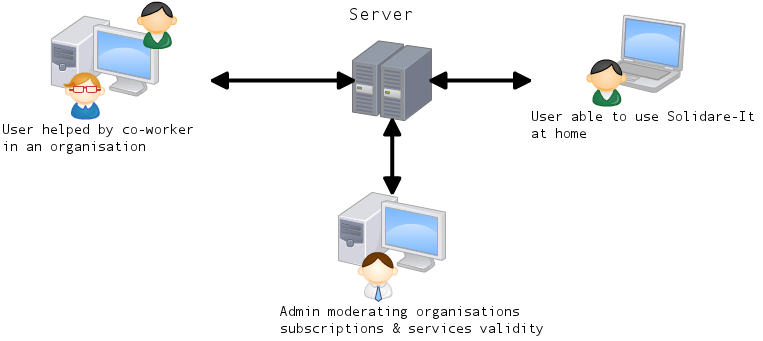
\includegraphics[width=\textwidth]{architectural_view_1.png}
		\caption{Website use}
		\label{fig:server}
	\end{center}
\end{figure}



\subsection{Pattern}
%– If applicable, a particular architectural style or pattern that is used. For example, it may be the case that the chosen web application framework imposes the use of a certain architectural pattern or architectural style (such as the model-view-controller architecture or MVC).

Ruby on Rails forces us to use the Model-View-Controller architectural style. Moreover, we all have experience with the MVC, then we will be more comfortable to code with this architecture.
\newpage

\section{Object Role Modeling}
\begin{center}
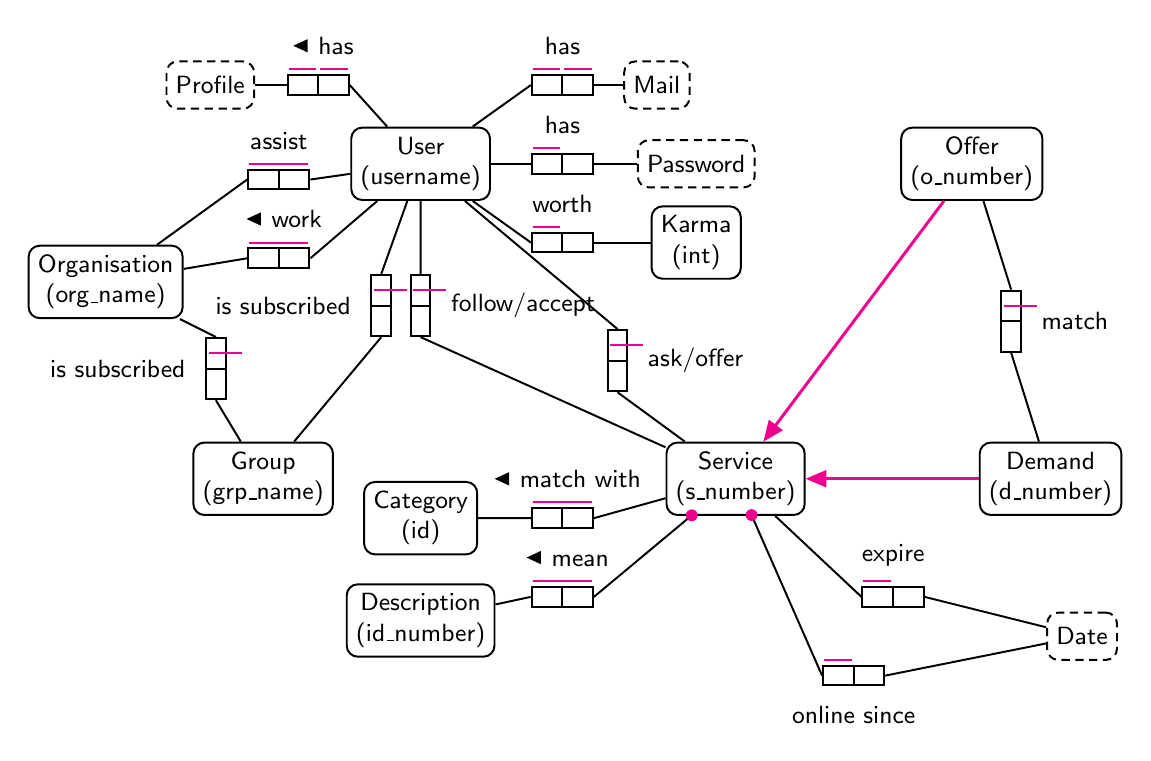
\begin{tikzpicture}[orm]

\entity (U) at (0,0) {User\\(username)};
 \binary[left= of U,  unique=1, unique=2, label=\ormleft{has}] (h) at (-0.5, 1) {};
 \value [left=of h] (Profile) {Profile};
 \plays  (U) to (h.east);
 \plays (h.west) to (Profile);
 
 
 \value (M) at (3,1) {Mail};	
 \binary [right=of U, unique=1, unique=2, label=has] (h2) at (1, 1) {};
 \plays (U) to (h2.west);
 \plays (h2.east) to (M);
 
 \value (Pa) at (3.5,0) {Password};	
 \binary [right=of U, unique= 1, label=has] (h3) at (1, 0) {};
 \plays (U) to (h3.west);
 \plays (h3.east) to (Pa);
 
 \entity (K) at (3.5, -1) {Karma\\(int)};	
 \binary [right=of U, unique= 1, label=worth] (h4) at (1, -1) {};
 \plays (U) to (h4.west);
 \plays (h4.east) to (K);
 
 \entity (Org) at (-4, -1.5) {Organisation\\(org\_name)};
 \binary [left=of U, unique=1-2, label=assist] (h5) at (-1, -0.2) {};
 \binary [left=of U, unique=1-2, label=\ormleft{work}] (h6) at (-1, -1.2) {};
 \vbinary [left=of U, unique=1-2, label=is subscribed] (h7) at (-2.2, -2.2) {}; 
 
 \plays (U) to (h5.east) (h5.west) to (Org) (U) to (h6.east) (h6.west) to (Org) (Org) to (h7.east);
 
 \entity (Gr) at (-2,-4) {Group\\(grp\_name)};
 \plays (h7.west) to (Gr);
 
 \vbinary [unique=1-2,label=is subscribed] (h8) at (-0.5,-1.8){};
 \plays (U) to (h8.east) (h8.west) to (Gr);
 
 \vbinary [unique=1-2,label=below:follow/accept] (h8bis) at (0,-1.8){};
 
 
 \entity (S) at (4, -4) {Service\\(s\_number)};
 \entity (O) at (7, 0) {Offer\\(o\_number)};
 \entity (D) at (8, -4) {Demand\\(d\_number)};
 \plays (U) to (h8bis.east) (h8bis.west) to (S);
 \vbinary [unique=1-2, label=below:ask/offer] (h9) at (2.5,-2.5) {};
 
 \plays (U) to (h9.east) (h9.west) to (S);
 
 \draw[subtype] (S) to (O);
 \draw[subtype] (S) to (D); 
 
 \vbinary [unique=1-2, label=below:match] (h10) at (7.5,-2){};
 \plays (O) to (h10.east) (D) to (h10.west);
 
 \entity (C) at (0, -4.5) {Category\\(id)};
 \entity (Desc) at (0, -5.8) {Description\\(id\_number)};
 
 \binary [unique=1-2, label=\ormleft{match with}] (h11) at (1.8, - 4.5) {};
 \binary [unique=1-2, label=\ormleft{mean}] (h12) at (1.8, - 5.5) {}; 
 
 \plays [mandatory] (S) to (h11.east) (S) to (h12.east); 
 \plays(h11.west) to (C) (h12.west) to (Desc);
 
 \value (Date) at (8.4,-6) {Date};	
 \binary [unique=1, label=expire] (h13) at (6,-5.5){};
 \binary [unique=1, label=below:online since] (h14) at (5.5,-6.5){}; 
 
 \plays (S) to (h13.west) (h13.east) to (Date) (h14.east) to (Date);
 \plays [mandatory] (S) to (h14.west);

\end{tikzpicture}
\end{center}


An ORM diagram is a diagram that modelises a database. It uses techniques of oriented object programming to define the 
database.

This one illustrates how we want to modelise our database for the SolidareIt website. There are three main entities. The first one is the users. As we saw in the class diagram above, users can be very different. There are co-workers, clients and simple users (using website on their own). The main fields of the user entity are mail, password and karma (based on other users evaluations). You can see that e-mail and password fields aren't mandatory. It's because a user can be created and handled by an organisation. So, in this case, the user account is minimal and there's no need for these fields. There's no rules to constraint group of fields. In our application, the constraint stands on User-Mail-Password or User-Profile-Organisation. During the creation of a user account by an organisation, the application will let the co-worker choose if the created user can have a full account or a minimal one. \texttt{Profile} entity regroups a few informations linked to the users and which are not imposed like the address, the firstname, the birthdate, etc. It also keep informations about the users status (client, co-worker, admin,etc.)\\
Services are the second main entity. We will extend it as an offer or a demand to make them more specific. To manage database more easily and to help keeping a trace of history, we want a match between offers and demands. This matches (if accepted by users of both sides) will stored in a transaction table, and as soon as the transaction happened, the entities will move in an history table. 
The third main entities are the organisations. They will store co-workers and clients related to them. We included the functionality for organisations to subscribe to a group. All co-workers of organisations involved in a group will be able to share informations, offers or demands with this group. Category table will be subdivised in two tables to add subcategories specified in the class diagram.





\newpage

\section{Development Plan}
In this section, we'll show you how we'll organize the implementation work of the web application. First, we'll decompose the implementation in several modules. Then, we'll organize it in a gantt diagram. \\

\subsection{Modules decomposition}
\begin{itemize}
\item a system kernel with object oriented model related with database, a base for pages display, utils functions
\item Connection/subscribing system
\item Search system
\item Account manager
\item Offer/Demand creator
\item Transaction aknowlegement
\item System related to organisations (user managing, offer/demand supervisor)
\item Group manager
\item E-mail and ID-cards validation
\end{itemize}

\subsection{Extensions}
In the previous report, we made the choice to implement an internal message service between the users to help to communicate while making transactions.There is a module in RoR which already implement this kind of service. We'll have to learn how to use it and put it into our application. \\

\subsection{Estimation and distribution of modules}
Since we choose a framework we didn't work with yet, it's difficult to know how much time will be needed to complete the first module (Kernel). After the development of this module, the others seems to have equivalent difficulty. It will be easier for us to share the work. We will not give now some specific modules to a specific group member. We will try to assign the modules in terms of each member qualifications.

\subsection{Gantt diagram}
\begin{figure}[!ht]
	\begin{center}
		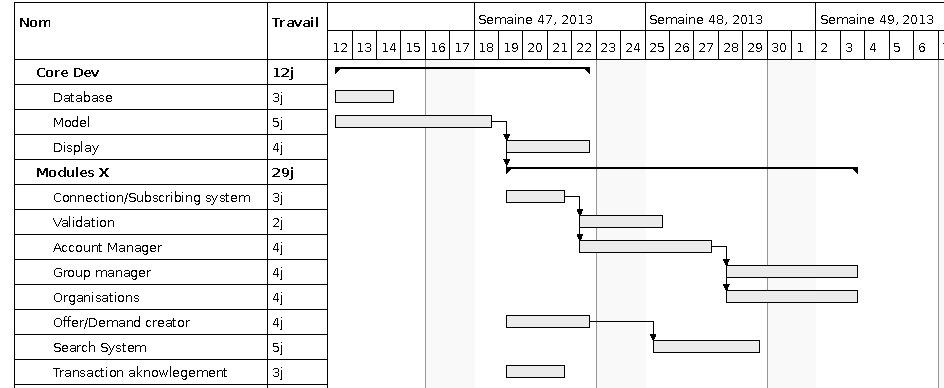
\includegraphics[width=\textwidth]{gantt_2_22_2_76.pdf}
		\caption{Gantt chart}
		\label{fig:gantt}
	\end{center}
\end{figure}
\newpage

\section{Framework}
\label{ror}
\subsection{Advantages of the framework}

We chose \emph{Ruby on Rails (RoR)} as framework for the project. After some research about existing frameworks, we found that RoR gives us many advantages. We have listed these pros here :

\begin{itemize}
   \item RoR constraints us to use the MVC design pattern which we are comfortable with.
   \item RoR forces us to apply good practices like "\emph{Don't repeat yourself}".
   \item RoR has conventions over configurations that allow us to waste less time configuring our project and making choices.
   \item RoR has an integrated structure. It allows us to have a clean code through the all project.
   \item RoR make easier to manipulate DB. So, it allows to reuse the same DB throughout all devices and platforms (mobile apps, etc.).
   \item RoR already contains development environment like \emph{production}, \emph{test} and \emph{development}. It makes the deployment easier.
   \item RoR provides protection tools against the most used security attacks. It's important in this case because the platform will contains some confidential informations about the users.
   \item RoR has a large active community of users. Then it is easier to find help and documentation. Moreover there
   are some \emph{gems}\footnote{\emph{gems} are packages for ruby programs and
   librairies.} availale to allow us to add some features very quickly 
   (like some extensions proposed like messaging service, connection service). 
   \item There's a lot of offers to host and deploy a RoR project. Moreover some are free to use and 
   propose all tools for a middle-sized website.  In addition, we found some maintenance tools like failures log or security tools.
\end{itemize}

In addition, lot of companies are looking for RoR developers. So, we're very interested in learning it. Moreover, 
some members of the group knew it already so they will be able to guide the rest of the group.

\subsection{Comparisons of the frameworks}

We chose Ruby on rails rather than other frameworks for multiples reasons.  
If we look at the languages used by the frameworks, we made the choice not to use PHP 
and Java.  PHP becomes less and less used by companies for web applications because it does not support new 
web features and a clear model programming.  For Java language, we didn't find a very good framework 
that allows to use all possibilities of Java.  Some years ago, Google develloped GWT, a good framework 
that transformed Java in Javascript but the programming model was too heavy to offer a new opportunity to 
use Java for web applications.  Moreover, with a Java web applications, we must use a server that allows 
Java and we did't find a good free offer for this kind of service.

In the languages that are not known by at least one member of the group, we found Smalltalk with 
Seaside framework.  After a first look at the Seaside website, we found a small community with not 
enough documentation and plugins.  Moreover, we didn't find a lot of websites based on Seaside.

We also looked the advantages of Django and really hesitated between Django and RoR. But we learned that
the Django documentation is smaller than the RoR one. So it's more difficult to discover it according to some articles found on the Internet. Moreover, we have to learn python this semester for other 
courses so it seemed more interesting to learn a new language.

\newpage
%\section{Activity Diagrams}
%\subsection{Welcome Page}

\begin{center}
	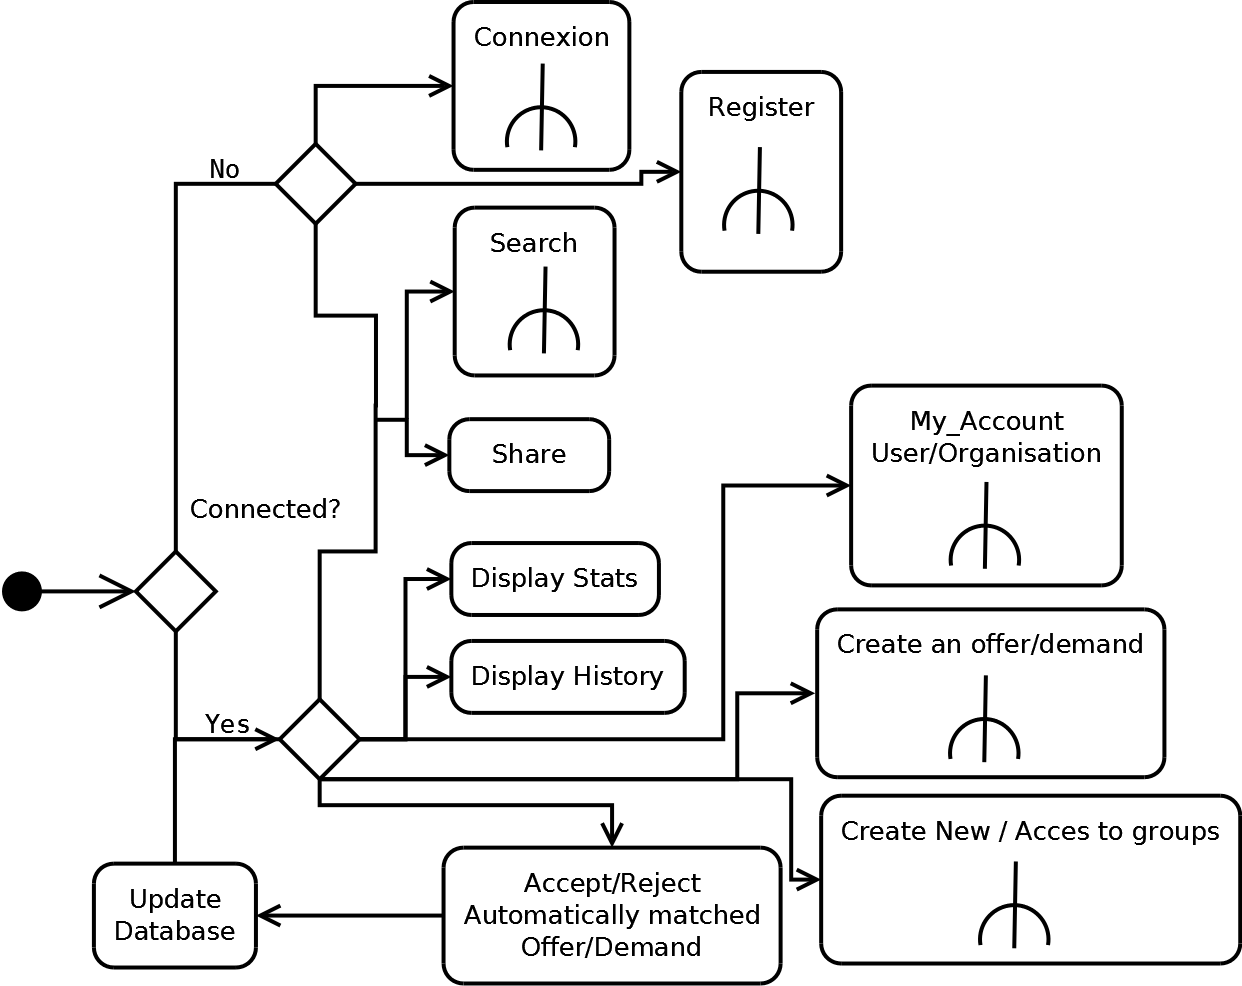
\includegraphics[width=.75\textwidth]{WelcomePage.png}
\end{center}
This diagram shows which functionalities are available to registered and unregistered users when they connect to the welcome page. If the user is logged in, the website displays the different matching that have been made since his last visit so that the user can accept or reject those propositions.

\subsection{Connexion}

\begin{center}
	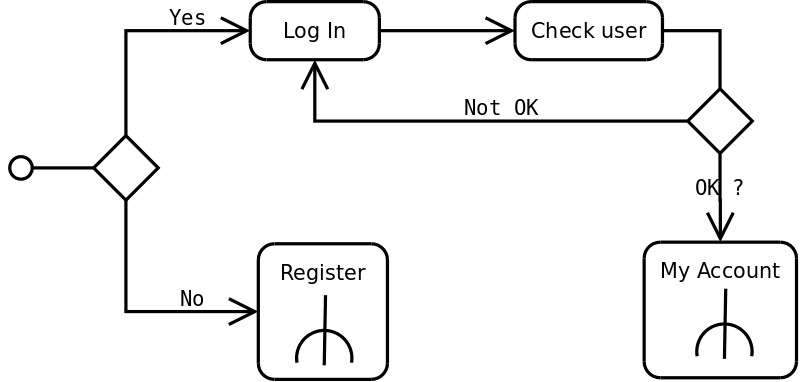
\includegraphics[width=.65\textwidth]{Connexion.png}
\end{center}
This diagram shows the interaction a user has with the website when he wants to be connected on the website.

\subsection{\texttt{MyAccount}: User}

\begin{center}
	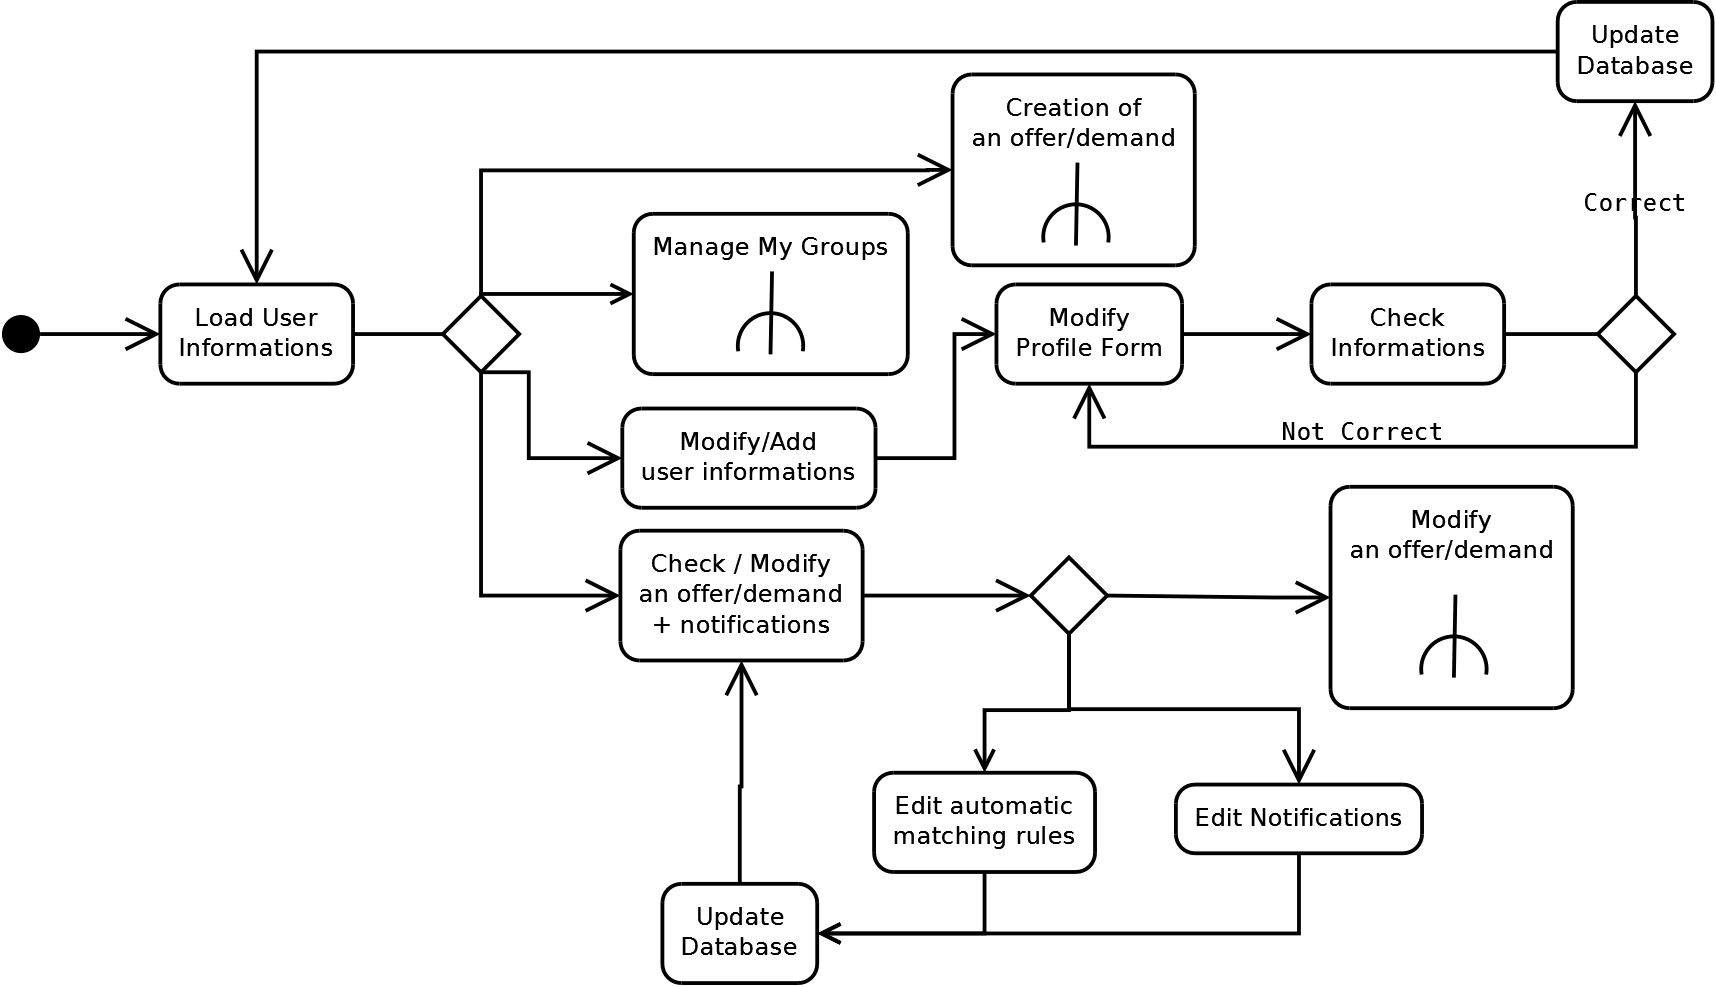
\includegraphics[width=1\textwidth]{MyAccount_User.png}
\end{center}
This diagram shows the possible interactions between a user and the website when he's on the main page after he log in. The user will be able to create a new offer/demand of services or to modify his profile informations. He can also manage offers/demands which he's subscribed to. The managing activity of groups is also made in this diagram.

\subsection{\texttt{MyAccount}: Organisation}

\begin{center}
	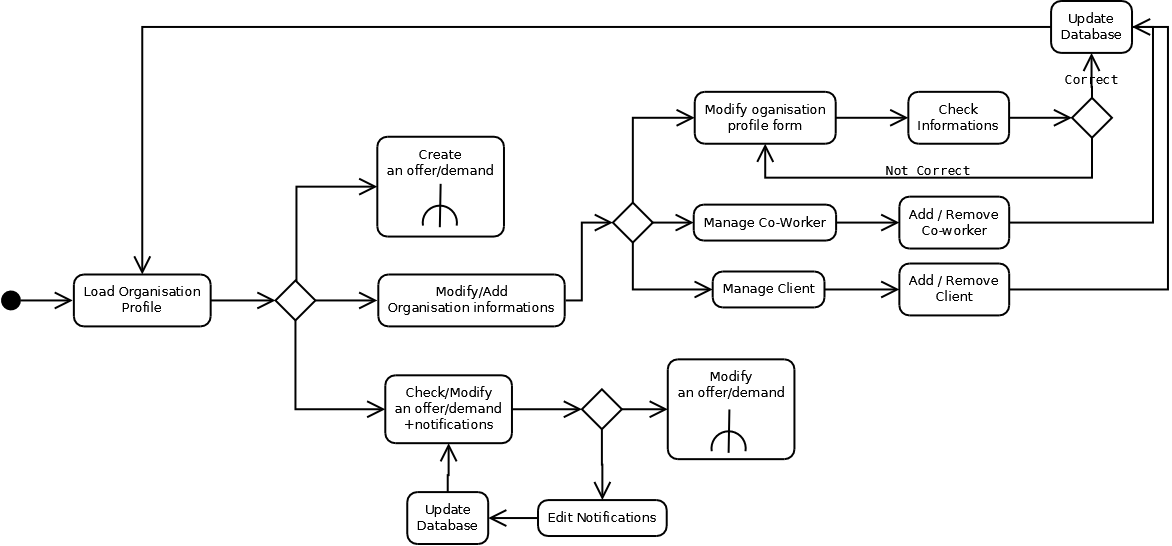
\includegraphics[width=1\textwidth]{MyAccount_Org.png}
\end{center}
Functionalities for organisations are basically the same as the ones for users. According to the requirements of the client, we will add functionalities to manage accounts of different clients (maybe people without any computer or internet connection at home), to create accounts for this clients and to manage a list of co-workers involved in the same organisation.

\subsection{Register}

\begin{center}
	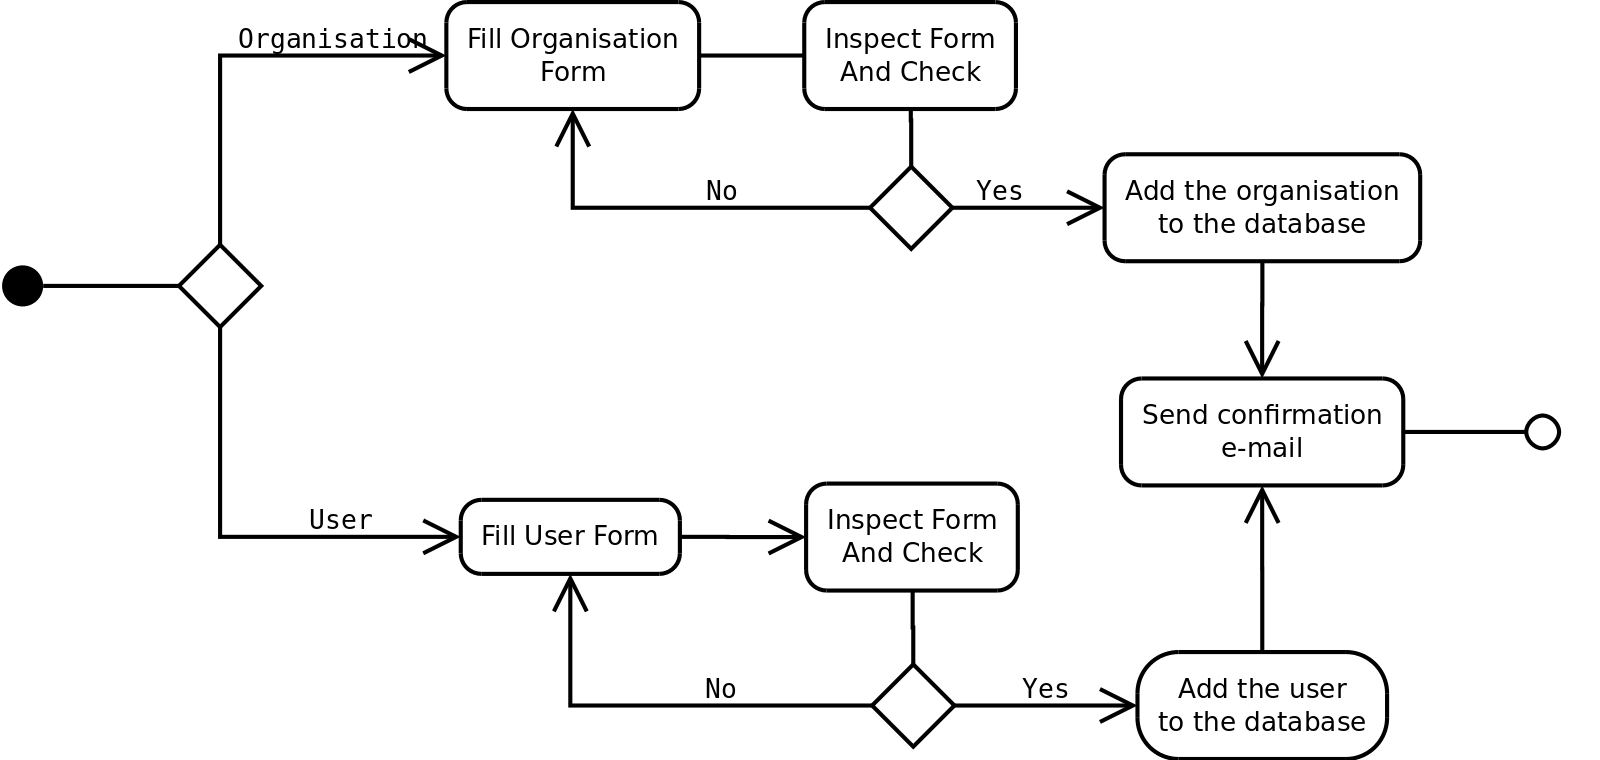
\includegraphics[width=.9\textwidth]{Register.png}
\end{center}
When a user wants to create an account, there are two possibilities:
\begin{itemize}
\item He can register as an organisation, there will be some checks to verify that it's a real social organisation. There will be a few more informations to give (like possible co-workers) into the form.
\item He can register as a user, either as a real user which need or provide service, or as a co-worker involved in an organisation. Co-workers profile are allowed only by an organisation.
\end{itemize}

\subsection{Group}

\begin{center}
	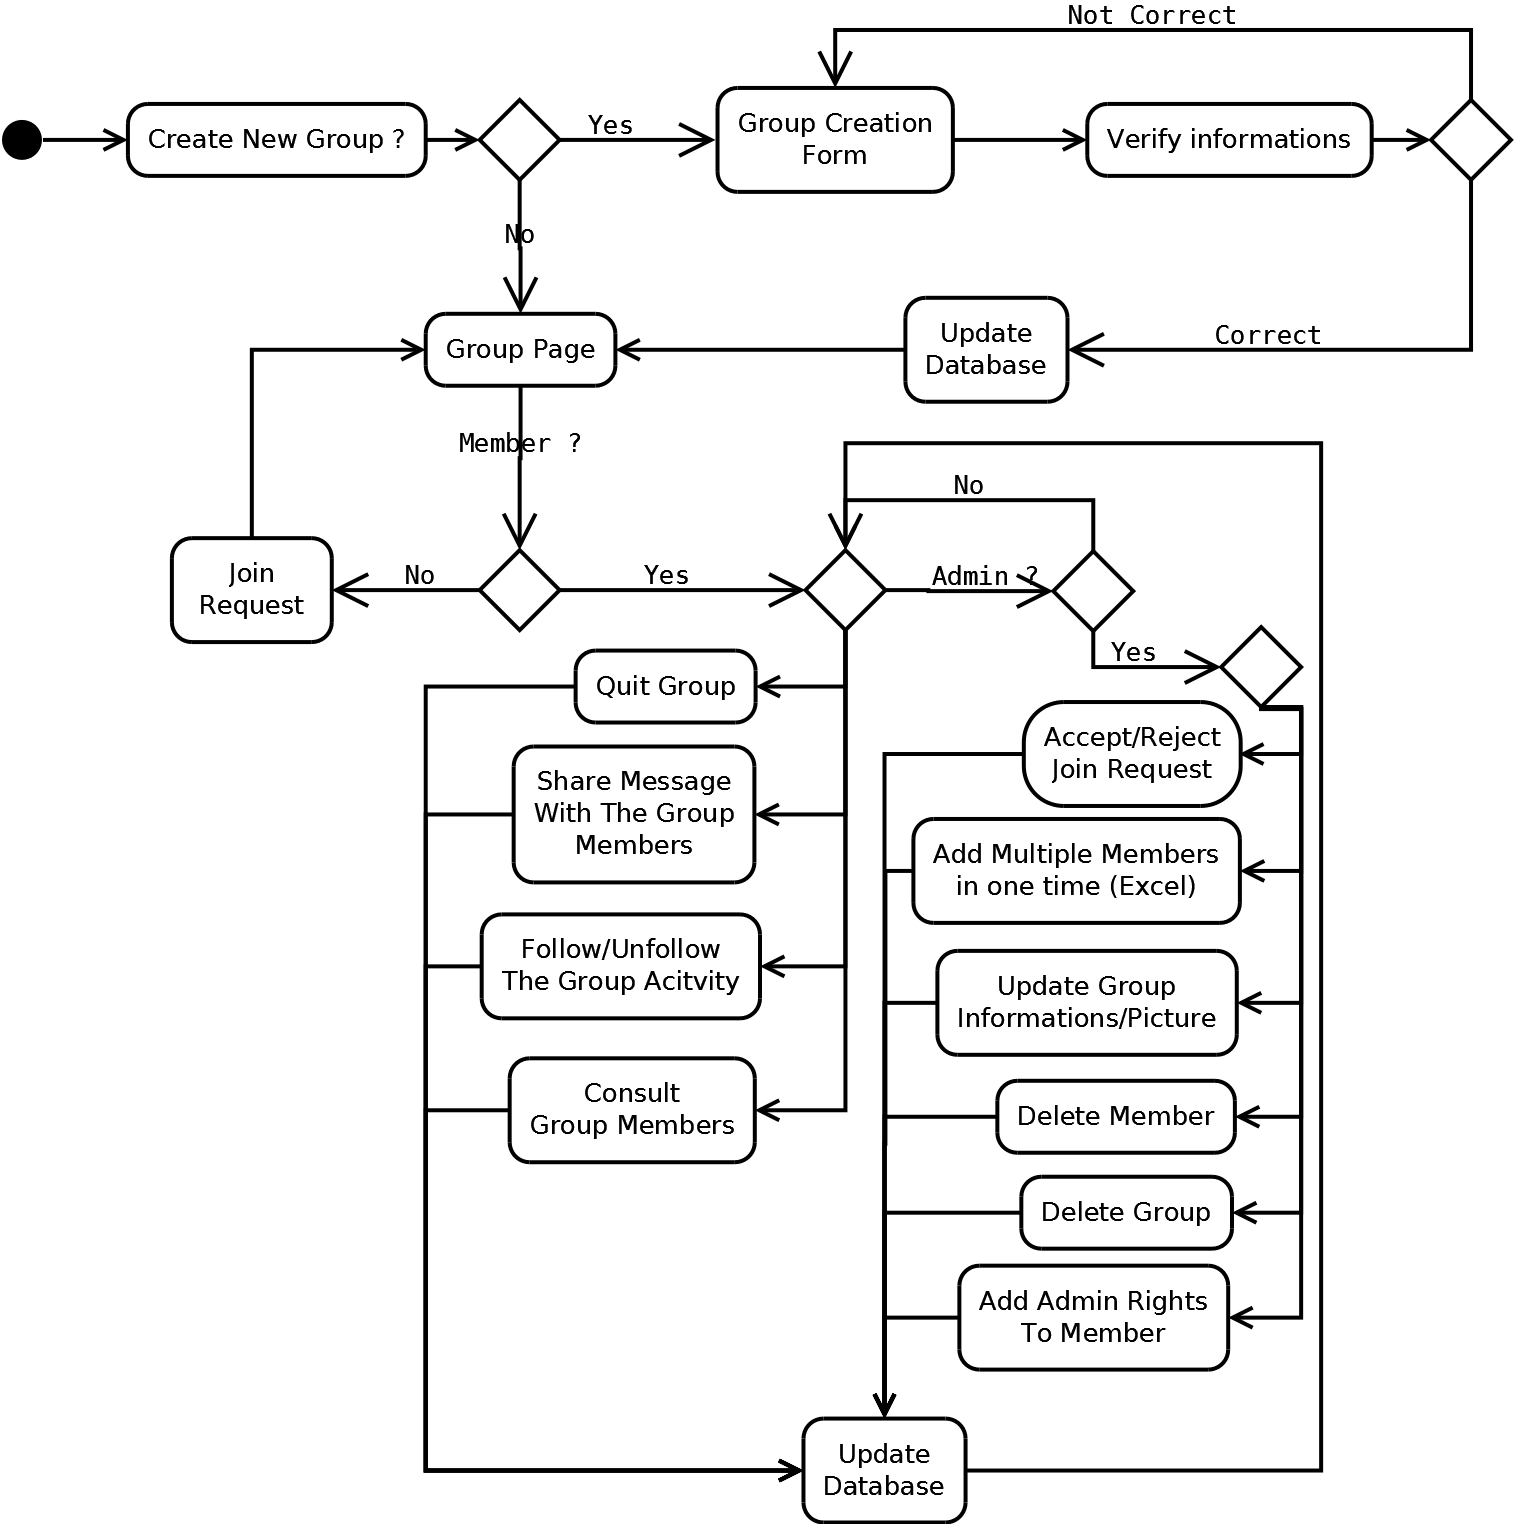
\includegraphics[width=.95\textwidth]{Group.png}
\end{center}
This diagram shows the different steps to create, manage and use a group, as an administrator and a (non) member of this group.

\subsection{Create or modify offers and demands}

\begin{center}
	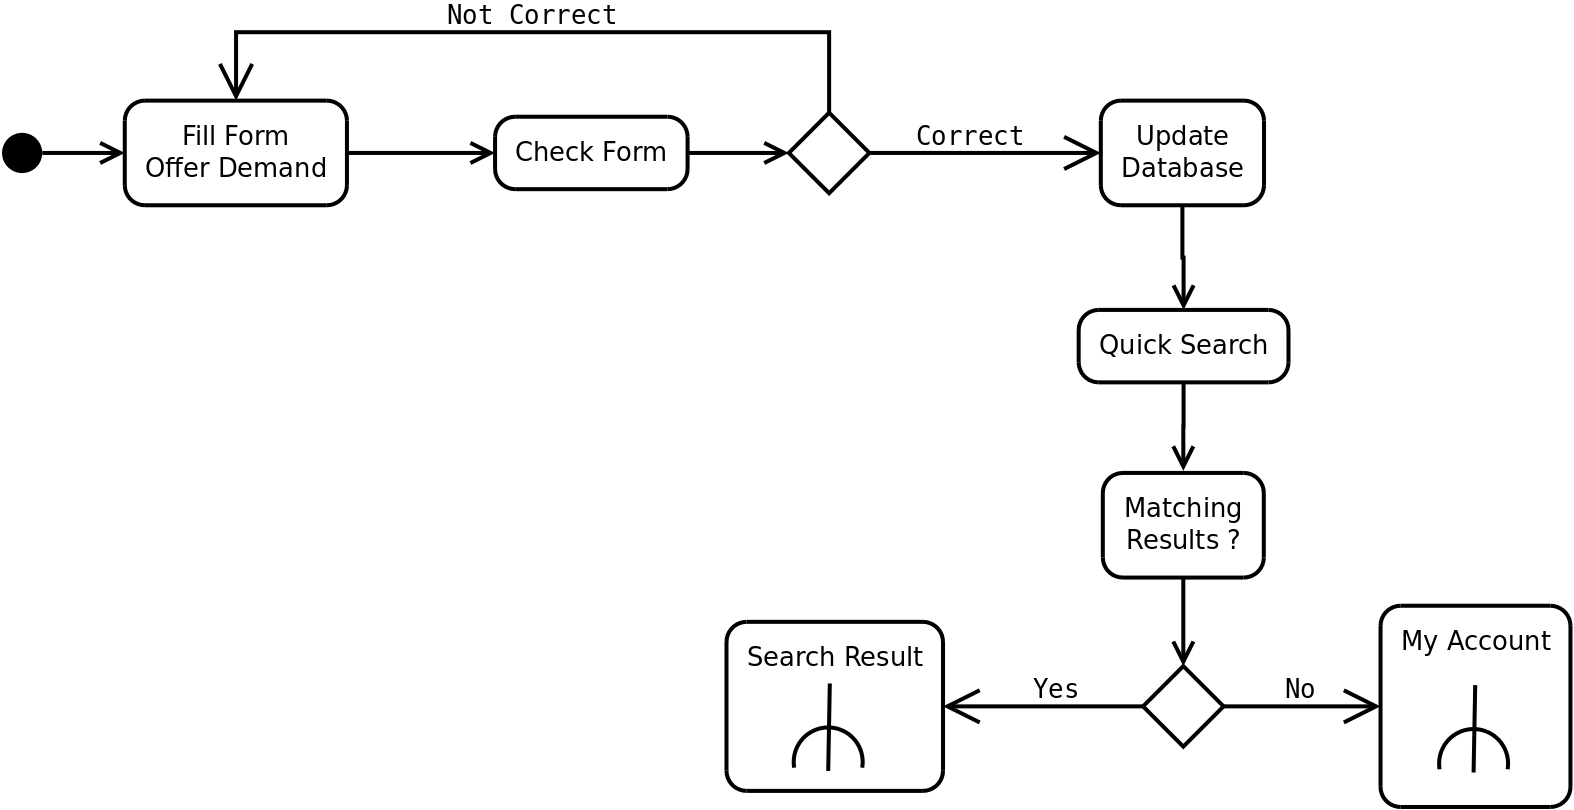
\includegraphics[width=.95\textwidth]{Create_Offer_Demand.png}
\end{center}
The user/organisation connected can at any moment create offers/demands of services. Organisation can create them for their clients. As soon as the offer/demand has been registered into the database, an immediate quick search is performed by the application. In case of successful search, results are automatically shown to the customer. Otherwise, the user is redirected to their account page.
As a standard user, you can also post a group offer/demand or an individual offer/demand.

\subsection{Search}

\begin{center}
	\hspace*{-1cm}
	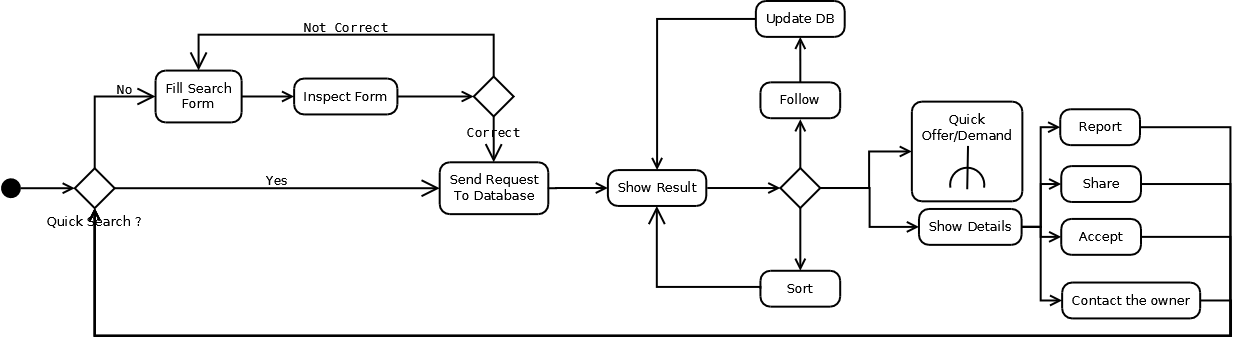
\includegraphics[width=1.1\textwidth]{Search.png}
\end{center}
There are two possible way to perform a search either on purpose (via the search button) or as the result of a matching while creating demand/offer. For each possible result, the customer can see the offer/demand's details individually, subscribe to one's he's interested in. If he wants to realise the service asked/offered, he can create a quick offer/demand which match the selected result. We assume that every demand as a corresponding offer and the opposite as well. 


\newpage
\section*{Conclusion}
\addcontentsline{toc}{section}{Conclusion}
This work was the occasion to learn on one hand about software technology and on the other to improve our working organisation in a larger team than usual.
On this phase, our leader took his job very seriously by organizing and leading in meetings.
We also are more efficient with our collaborative development tools Trello and writeLatex.\\

We improve our experience of separating the work that has to be done in different parts.
We had to give back a consistent report so communication between us becomes really important.
To reach the goal before the deadline, we had to separate the job in different tasks attributed to subgroups.
In these subgroups working on different diagrams, we can still create responsibilities like two persons drawing the diagram on a white board and the third one transcript it into virtual file usable on the computer.\\

Now that we have a better module decomposition, we have a view on the time required to achieve this project.
The module decomposition allows us to improve the separation of the responsibilities. We hope that we gave you a better look on the project.
We have now a clear idea on what the application will be.
On development part, we have already thought about the minimal requirements of this architecture and we have also some ideas in our pockets to push the application .


%%We learn to DO NOT put exclamation mark in a technical document!


% \label{LastPageModif}

\newpage

\appendix
\section{Diagrams}

The diagram on Figure 3 shows what happens when a user is interested by a service. First the user click on the 'Accept' button of this service (aService in the Figure 3), then we add this user in the list of users interested in this service.
\\ If this user is the first on this list, the server do a transaction, update the service then we add this transaction to the "transactions historic" of both the user and the creator of this service.
\\ Finally, we send a message from the customer to the creator to let him know his interest. We do this in every case because we want to let the creator know about all the followers. It can be interesting, for example, if the first customer of the list didn't manifest after a long time, the creator know the other customer and then can contact them.

\begin{figure}[!ht]
	\begin{center}
		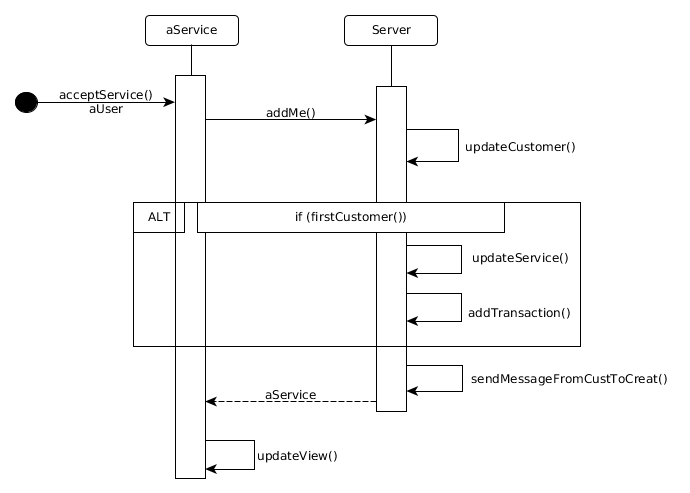
\includegraphics[width=\textwidth]{seq_acceptService.png}
		\caption{Sequence Diagram : Acceptance of an offer or a demand}
		\label{fig:acceptService}
	\end{center}
\end{figure}

The diagram on Figure 4 shows what happens when a user creates a service (an offer or a demand). After fulfilling the form and checking the integrity of the form. We send to the server the date, the server will then send an object service (aService in the Figure 4). We then give to the creator the opportunity of sharing this service with an eventual group and/or on a social network. 
\\ Meanwhile, we will do an automatic search to see if there is already an offer/demand in the database that can match this new service and show the results to the creator.

\begin{figure}[!ht]
	\begin{center}
		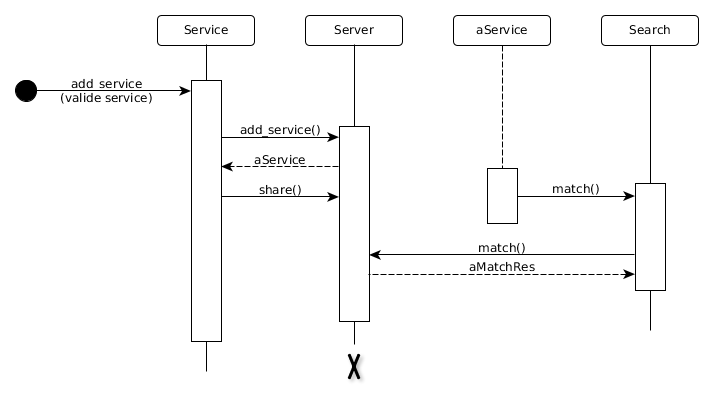
\includegraphics[width=\textwidth]{seq_addService.png}
		\caption{Sequence Diagram : Creation of an offer or a demand}
		\label{fig:addService}
	\end{center}
\end{figure}

\newpage
In the Figure 5, we show the creation of a user account on the website. An unregistered user, after fulfilling the form and after we check its integrity, push the "create Account" button. We send the data from the form to the server, the server then add this new user to the DataBase. 
\\ Then, it sends back a 'user object', an object that contains all the information that the user gives us plus his ID. With this information, we can show the Profile of the user.

\begin{figure}[!ht]
	\begin{center}
		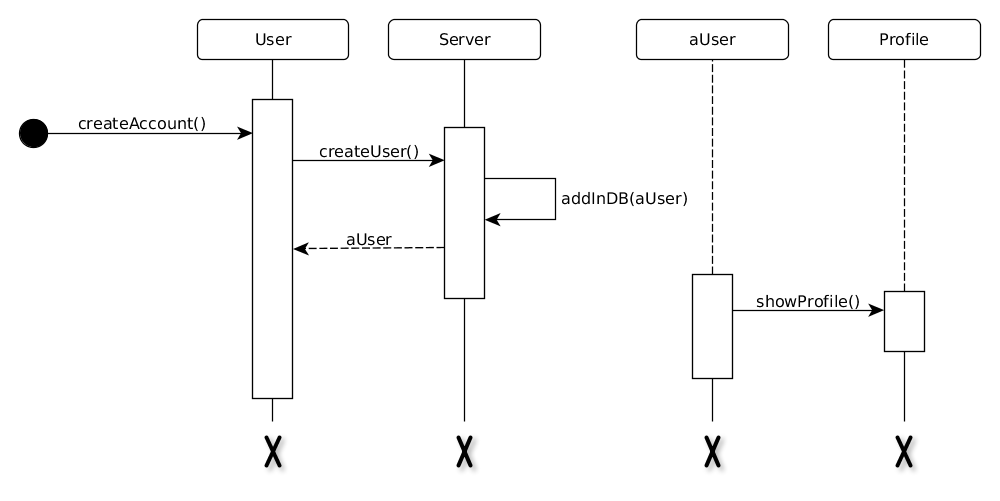
\includegraphics[width=\textwidth]{seq_createUser.png}
		\caption{Sequence Diagram : Creation of an account on the website}
		\label{fig:createUser}
	\end{center}
\end{figure}

In the Figure 6, we show the possibilities give to the user when he perform a search. After taking the data from the search form, the server performs a match and send back the results.
Once we have the results, we can do several things.
\begin{itemize}
	\item SORTED : With this action, the user can order the results by differents fields (date, creator, title, tag, ...)  in a decreasing or increasing order. We order in a dynamic way in this way we have less request on the server.
    \item FOLLOW : With this action, the user can add himself in the list of the followers of this service. A follower is always informed of the modifications on the service.
    \item QUICKS : With this action, the user can accept a service.  In our server, we perform this action by adding a new service that match with the request of the user.  After that, we perform the sames actions that we explain in Figure 1 : accept a service.
    
\end{itemize}

\begin{figure}[!ht]
	\begin{center}
		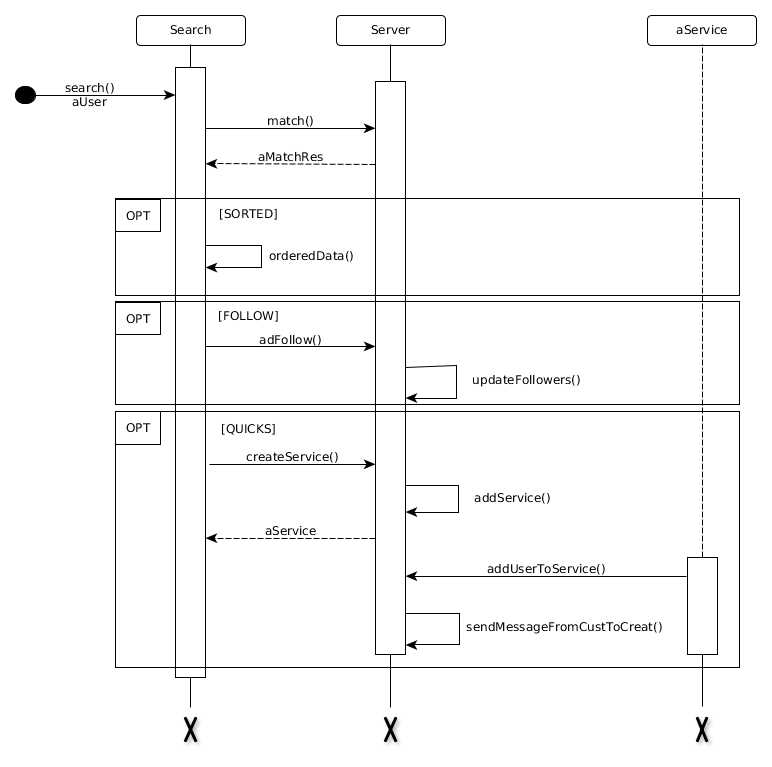
\includegraphics[width=\textwidth]{seq_search.png}
		\caption{Sequence Diagram : The procedure of a search}
		\label{fig:search}
	\end{center}
\end{figure}

On the Figure 7, we show what happens when a service is finished, ie when the customer and the creator met and performed the service.
\\ When it's finished, the creator and/or the customer can send a cotation with a optional message. 
\\ We get this informations from a form, the server then update the service, add karma (ie the cotation) to the customer or the creator and add the message to the 'transactions history' of the customer or creator.
\\ If the customer and the creator have given a cotation, we ask to server the list of all other user interested by the service and send them a message to warn them that the offer/demande is not available anymore. After that, we archive the service.
\\ If the customer or the creator didn't give a cotation, we send them a message and ask them to give one as soon as possible.

\begin{figure}[!ht]
	\begin{center}
		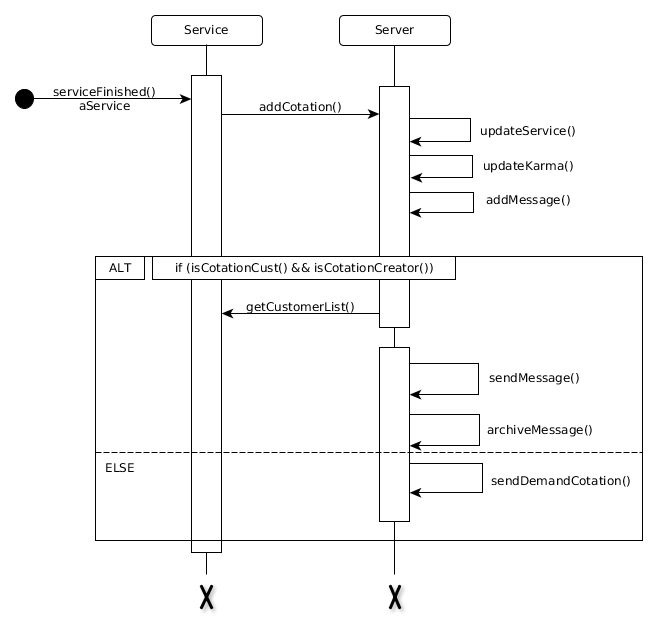
\includegraphics[width=\textwidth]{seq_serviceFinished.png}
		\caption{Sequence Diagram : End of a Service, Cotation and Karma}
		\label{fig:serviceFinished}
	\end{center}
\end{figure}


\begin{landscape}

\begin{figure}[!ht]
	\begin{center}
		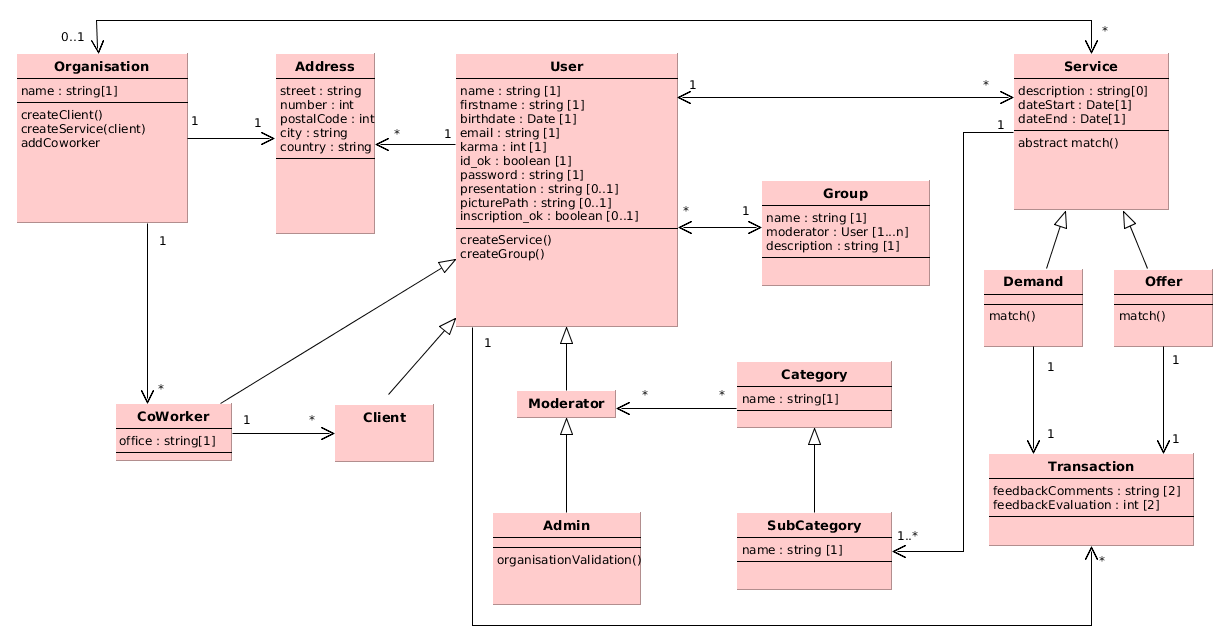
\includegraphics[width=.85\paperheight]{UML.png}
		\caption{Unified Modeling Language (UML): class diagram}
		\label{fig:uml}
	\end{center}
\end{figure}


\end{landscape}


\end{document}